\chapter{Anforderungen}
\label{chapter-analyse}

Um Benutzende, Aufgaben und Kontext des Projektes genauer zu verstehen, wurde eine Analyse nach dem
menschenzentrierten Gestaltungsprozess durchgeführt \cite{DINISO9241}.
Hierbei wurden relevante Anforderungen, die Einfluss auf die Entwicklung und die spätere Nutzung des
Reservierungstools nehmen, identifiziert und eingeordnet. Mit der Durchführung einer Recherche,
welche in den Datenquellen (\ref{section:daten}) genauer präsentiert wird, wurden zunächst zwei
Benutzergruppen (Verleihende und Ausleihende) festgehalten. Mittels einer Benutzeranalyse
(\ref{section:benutzer}) unter der Zuhilfenahme von durchgeführten Interviews, konnten diese weiter
klassifiziert und eingegrenzt werden. Daraufhin wurden die Probleme und Herausforderungen des
aktuellen Vorgehens und den unterschiedlichen Ausleihprozessen (\ref{section:iststand}) hergeleitet.
Anschließend wurden die Aufgaben, die Verleihende und Ausleihende mithilfe der Anwendung bewältigen
sollten, diskutiert (\ref{section:aufgaben}). Abschließend wurde der organisatorische und
zeitlich-räumliche Kontext des Verleihens und Ausleihens am \ac{imis} (\ref{section:kontext})
untersucht. Aufbauend auf den Resultaten der vorangestellten Untersuchungen wurden die objektiven
Anforderungen an den Snipe-IT Companion nach \citeA{Balzert2009} formalisiert
(\ref{section:anforderung}). Diese dienen als Grundlage für das gesamte Konzept der Arbeit.

\section{Datenquellen}
\label{section:daten}
Im Rahmen der Analyse wurden \nameref{subsection:interview} durchgeführt (\ref{subsection:interview}).
Darauffolgend wurde nach vergleichbaren Projekten und Systemen recherchiert
(\ref{subsection:system}).

\subsection{Stakeholder-Interviews}
\label{subsection:interview}
Zunächst wurde anhand der zu untersuchenden Gesichtspunkte ein Interviewleitfaden für ein
semi-strukturiertes Interview entwickelt (\ref{appendix-analyse-interview}). Mithilfe dieses Leitfadens wurden die Befragten
durch das Interview geführt. Die Interviews wurden aufgezeichnet und anschließend in Teilen,
mithilfe eines vereinfachten Transkriptionssystems, verschriftlicht \cite{dresing_praxisbuch_2016}. Daraufhin wurde eine
qualitative Inhaltsanalyse durchgeführt. Hierfür wurden die Transkripte erneut gelesen und für die
Arbeit und Forschungsfragen relevante Textstellen kommentiert. Infolgedessen wurden die erarbeiteten
Kommentare in ein Ordnungssystem strukturiert und unter den einzelnen Analysepunkten zusammengefasst
\cite{dresing_praxisbuch_2016}.

Es wurde eine Unterteilung in Verleihende und Ausleihende von Assets vorgenommen (genauere
Definition der Benutzergruppen in \ref{section:benutzer}). Bei den Teilnehmenden handelt es sich um
Mitarbeitende, welche am \ac{imis} tätig sind und Studierende der Medieninformatik an der
Universität zu Lübeck. In \ref{table:v} ist der jeweilige (Haupt-)Zuständigkeitsbereich der
Verleihenden aufgeführt. Verleihende der Assets können gleichzeitig die Position eines Ausleihenden
einnehmen. Die Ausleihenden umfassen außerdem Studierende, welche in \ref{table:a} dargestellt sind.
Durch den geplanten Einsatz am \ac{imis} wurde sich zunächst ausschließlich auf \ac{wimi} des
\ac{imis} und Studierende der Medieninformatik begrenzt. Hierbei wurde insbesondere der Fokus auf
die Probleme am \ac{imis} gelegt (genauere Untersuchungen in der Problemanalyse in
\ref{section:iststand}). Die IDs der Teilnehmenden werden als Verweise in den folgenden Abschnitten
verwendet.

Des Weiteren wurde mithilfe des \ac{ati} das technische Interesse und Verständnis der Teilnehmenden
festgestellt (\ref{table:ati}) \cite{attig_assessing_2017}.

\begin{table}[h]
        \centering
        \caption{Teilnehmende der Interviews, Verleihende}
        \begin{tabular}{lll}
                \arrayrulecolor{maincolor}\hline
                \sffamily\color{maincolor}ID & \sffamily\color{maincolor}Alter &
                \sffamily\color{maincolor}Zuständigkeitsbereich                                   \\
                \arrayrulecolor{maincolor}\hline
                V1                           & 25 - 35 J.                      & Keine direkte
                Zuständigkeit, Zugänge zu verschiedenen Laboren                                   \\
                V2                           & 25 - 35 J.                      & Multimedialabor
                \\
                V3                           & 25 - 35 J.                      & VR-Labor
                \\
                V4                           & 40 - 59 J.                      & Administratives
                Personal                                                                          \\
                V5                           & 25 - 35 J.                      & Innovationslabor
                \\
                \arrayrulecolor{maincolor}\hline
        \end{tabular}
        \label{table:v}
\end{table}

\begin{table}[h]
        \centering
        \caption{Teilnehmende der Interviews, Ausleihende \\
                (die mit * gekennzeichneten Personen wurden gemeinsam interviewt)}
        \begin{tabular}{lll}
                \arrayrulecolor{maincolor}\hline
                \sffamily\color{maincolor}ID & \sffamily\color{maincolor}Alter &
                \sffamily\color{maincolor}Rolle                                                     \\
                \arrayrulecolor{maincolor}\hline
                A1                           & 19 - 25 J.                      & Bachelorstudentin,
                Hilfswissenschaftlerin                                                              \\
                A2                           & 19 - 25 J.                      & Bachelorstudent
                \\
                A3                           & 19 - 25 J.                      & Masterstudent,
                Hilfswissenschaftler                                                                \\
                A4*                          & 19 - 25 J.                      & Bachelorstudentin
                \\
                A5*                          & 19 - 25 J.                      & Bachelorstudentin
                \\
                A6                           & 19 - 25 J.                      & Masterstudentin
                \\
                \arrayrulecolor{maincolor}\hline
        \end{tabular}
        \label{table:a}
\end{table}


\begin{table}[h]
        \centering
        \caption{Werte der \ac{ati}-Skala}
        \begin{tabular}{lccc}
                \arrayrulecolor{maincolor}\hline
                \sffamily\color{maincolor}Benutzergruppe & \sffamily\color{maincolor}Mittelwert
                $(M)$                                    & \sffamily\color{maincolor}Standardabweichung $(SD)$ &
                \sffamily\color{maincolor}Teilnehmende $(N)$                                                          \\
                \arrayrulecolor{maincolor}\hline
                Verleihende                              & 5,00                                                & 0,58
                                                         & 3                                                          \\
                Ausleihende                              & 5,13                                                & 0,48
                                                         & 6                                                          \\
                \arrayrulecolor{maincolor}\hline
        \end{tabular}
        \label{table:ati}
\end{table}

\subsection{Recherche vergleichbare Systeme}
\label{subsection:system}
Für die Recherche wurden die digitalen Bibliotheken ACM Digital
Library\footnote{\url{https://dl.acm.org/}} und Google
Scholar\footnote{\url{https://scholar.google.de/}} genutzt. Es wurden Begriffe aus den Bereichen
Managementsystem \textit{(Assets, Assetmanagement, schedule)} und Reservation \textit{(reservation,
Lending, lend, borrow)} zur Suche verwendet. Die Recherche sollte dem besseren Vergleichen und
Abwägen der analysierten Interview-Ergebnisse dienen und vergleichbare Systeme und Projekte
eruieren. Des Weiteren sollte die Recherche dazu dienen mögliche Fehlerquellen zu erörtern, um diese
umgehen zu können. Durch den speziellen Einsatzort am \ac{imis} stellte sich zeitnah heraus, dass
wenige bis keine vergleichbaren Systeme gefunden werden konnten. Folglich boten die vorhanden
Vergleiche keinen hilfreichen Aufschluss für den Rahmen dieser Arbeit, daher wurde die Recherche
nicht fortgeführt.\todo{Systeme schildern}

% Vielleicht schilderst du lieber erst die zwei Beispiele und leitest dann ab, dass diese deinem Nutzungskontext nicht entsprechen und du demzufolge nur jene und solche Ableitungen treffen konntest?  Denke nur ans Kolloquium und mit so einer Aussage machst du dich relativ angreifbar, glaube ich 

\section{Benutzeranalyse}
\label{section:benutzer}
Um eine zielgruppengerechte Gestaltung des Snipe-IT Companion voraussetzen zu können, werden in
diesem Abschnitt die Benutzergruppen des Reservierungstools eruiert und näher untersucht.
Resultierend aus den Stakeholder-Interviews wurden zwei Benutzergruppen, zu denen Verleihende sowie
Ausleihende eines Assets gehören, für das System erarbeitet. Die Zielgruppe beschränkt sich im
Rahmen dieser Arbeit auf die Mitarbeitenden des \ac{imis} sowie die Studierenden der
Medieninformatik an der Universität zu Lübeck. Für den Snipe-IT Companion konnte eine Zielgruppe mit
einer Alterspanne von 17 - 35 Jahren festgelegt werden. Aus den Interviews (\ref{section:daten})
konnte entnommen werden, dass beide Benutzergruppen täglich ein Smartphone, Tablet, Laptop oder
Desktop PC nutzen und somit ein grundlegendes technisches Verständnis vorausgesetzt werden kann.
Diese Behauptung konnte mit den Ergebnissen der \ac{ati}-Skala bestärkt werden (\ref{table:ati}).


%Mitarbeitende, sowie administratives Personal des \ac{imis}, welche verantwortlich für die Ausgabe
%von Assets sind, werden im folgenden als Verleihende bezeichnet (\ref{table:v}).
\subsection{Verleihende}
Die Verleihenden eines Assets unterscheiden sich gering bis gar nicht in ihren soziodemografischen
Daten. Im Kontext der vorliegenden Arbeit sind besonders Technikaffinität und Alter zu beachten.

Mit $N=3$ und einem durchschnittlichen Alter von XX lag der Wert der \ac{ati}-Skala, aufseiten der
Verleihenden, bei $M=5,00$ mit $SD=0,58$. Dies weist auf eine hohe Technikaffinität hin
(\ref{table:ati}).

\cite{franke_personal_2019}
https://doi.org/10.1080/10447318.2018.1456150 \todo[inline]{Ohne Vergleich kann man bei einer Skala
        immer schwer sagen, ob der Wert nun hoch oder niedrig ist. Denn eine Skala muss nicht
        notwendigerweise normiert sein, das heißt, dass der theoretische Mittelwert einer Skala nicht dem
        Durchschnittswert der Normalbevölkerung widerspiegelt. Deshalb gibt es in der Psychologie, wenn
        einem Vergleiche fehlen, oftmals Vergleichsstichproben, die ein Gefühl dafür geben sollen, wie der
        Wert so bei anderen Studien war. Und wenn dann der eigene Wert darüber liegt, dann kann man fundiert
        sagen, dass man eine hohe Technikaffinität hat. :D Schaue mal in das Paper rein, da sind viele
        Vergleichsstichproben}

Die \ac{wimi} mit einem Zuständigkeitsbereich für Assets lagen im Großteil bei einer
Alterspanne von 25 - 35 Jahren. Folglich lässt sich eine Alterspanne von 25 - 35 Jahren aufseiten
der \ac{wimi} für den Snipe-IT Companion festlegen.

Verleihende umfassen ausschließlich Mitarbeitende, sowie administratives Personal des \ac{imis},
welche verantwortlich für die Ausgabe von Assets sind (\ref{table:v}). Allerdings haben nicht alle
Verleihende auf alle Assets den gleichen Zugriff, da dies von Forschungsgruppe zu Forschungsgruppe
unterschiedlich ist. Zudem liegen in den Forschungsgruppen unterschiedliche Vorgänge vor (genauere
Unterschiede zu den Vorgängen in \ref{section:iststand}). Folglich können Verleihende der Assets
gleichzeitig die Position der Ausleihenden einnehmen.

\subsection{Ausleihende}
Die Ausleihenden eines Assets unterscheiden sich systemseitig in ihren
soziodemografischen Daten kaum. Im Kontext der vorliegenden Arbeit sind besonders Technikaffinität
und Alter zu beachten.
\todo[]{Alle, also N 9}
Mit $N=9$ und einem durchschnittlichen Alter von XX lag der Wert der \ac{ati}-Skala, aufseiten der
Ausleihenden, bei $M=5,13$ mit $SD=0,48$. Dies weist auf eine hohe Technikaffinität hin
(\ref{table:ati}).

Das Alter der studierenden Deutschen betrug im Sommersemester 2012 im Durchschnitt 24,4 Jahre
\cite{middendorff2017wirtschaftliche}. In den Jahren 2019/20 lag das Durchschnittsalter der
insgesamt 2,9 Millionen Studierenden bei 23,4 Jahren \cite{noauthor_studierende_nodate}. Mit einem
durchschnittlichen Alter von XX der befragten Personen lässt sich eine Alterspanne von 17 - 25
Jahren aufseiten der Studierenden für den Snipe-IT Companion festlegen.

Bei den Ausleihenden handelt es sich insbesondere um Studierende, welche keinen direkten Zugang zu
den Assets haben (\ref{table:a}). Ausleihende suchen Verleihende (Mitarbeitende) aktiv auf oder
kontaktieren jene, um Informationen über ausleihbare Assets zu erhalten. Wie bereits geschildert,
können durch die Forschungsgruppen auch Verleihende zu Ausleihenden werden, wobei
für diese häufig ein anderer Ausleihprozess als für Studierende vorliegt (\ref{section:iststand}).


\section{Problemanalyse}
\label{section:iststand}

Um die Relevanz des Verleihens am \ac{imis} sowie die Prozesse und die damit einhergehenden
Problematiken besser nachvollziehen zu können, wurde eine Problemanalyse auf Basis des aktuellen
Vorgehens durchgeführt. Hierfür wurde sich auf die in \ref{section:daten} aufgeführten
Interview-Teilnehmenden referenziert. Der Übersichtlichkeit wegen werden zunächst Probleme,
welche Verleihende und Ausleihende betreffen, thematisiert. Daraufhin werden Probleme der einzelnen
Benutzergruppen näher erläutert.

\subsection{Probleme: Allgemein}
\label{section:probleme-allgemein}
Eines der größten Probleme im derzeitigen Ablauf ist das Nichtvorhandensein einer öffentlichen Liste
für Studierende, über die ausleihbare Assets eingesehen werden können. Auch aufseiten der
Verleihenden ist keine vollständige interne Übersicht vorhanden (V1-5, A1-6). Dies führt dazu, dass
aufgrund von fehlender Information wenig Assets ausgeliehen werden können (V1-5). Durch die verschiedenen
Forschungsgruppen am \ac{imis} und die damit verbundenen Labore, gibt es verschiedene
Ansprechpartner:innen für die jeweiligen Assets in den Laboren. Die Verantwortlichkeiten dieser
Ansprechpartner:innen ist jedoch nicht ausreichend ersichtlich, sodass es häufig zu Weiterverweisen
an andere Ansprechpartner:innen kommt, wobei auch unter den \ac{wimi} nicht immer
die Verantwortlichkeiten bekannt sind (V1,V3, V4, A1, A2, A3).

Studierende, welche als \ac{hiwi} am \ac{imis} angestellt sind, haben beim Ausleihen häufig einen
Vertrauensvorschuss, sodass bei kurzer Ausleihe für Tätigkeiten im Gebäude Assets verliehen oder
entnommen werden, ohne dies zu Vermerken. Diese Praxis gilt auch für \ac{wimi} (A1, V1, V2), wobei
das Planen mit Assets dadurch erschwert wird (A3, A6).

Beim Verleihen von Assets kommt es häufig vor, dass insbesondere Studierende ohne Erfahrungen und
Expertise ein Asset ausleihen wollen (V2, A3, A6). Folglich kann dies schnell zu Problemen führen.
Während einige Verleihende auf die Selbstaneignung und Google verweisen, ist es anderen wichtig, den
Use Case der Nutzung zu verstehen und die damit verbundenen Einstellungen der Assets sowie weiteres
Zubehör zu empfehlen (V1, V2, V4, V5). Somit ist die Nutzung der Assets durch das Ungleichgewicht
aufseiten der Verleihenden nicht kontrollierbar. Dies führt untereinander dazu, dass Beschädigungen,
Gebrauchsspuren und Mängel von Assets nicht festgehalten werden können. Ausleihende erfahren den
Zustand und die Mängel eines Assets erst zum Zeitpunkt der Abholung, was die Nutzung beeinträchtigen
kann (A1, V1, V5).

\subsection{Probleme: Verleihende}
\label{section:probleme-verleihende}
Eine zentrale Schwachstelle des aktuellen Vorgehens sind die uneinheitlichen Prozesse. Das Ausleihen
von Assets wird von Forschungsgruppe zu Forschungsgruppe unterschiedlich gehandhabt. Zudem liegen
auch innerhalb der Forschungsgruppen Unterschiede im Prozess vor (V1, V2, V3). Wie bereits in den
Allgemeinen Problemen (\ref{section:probleme-allgemein}) geschildert, ist es einigen Verleihenden
wichtig, dass Ausleihende über die Assets Bescheid wissen und der Use Case detailliert besprochen
und erläutert wird. Für andere ist die Vermittlung dieses Wissens wiederum nicht von Bedeutung
(V1, V2, V3, V4) (siehe Probleme: Ausleihende).

Um ein Asset ausleihen zu können, müssen Ausleihende, je nach Zuständigkeitsbereich, entweder ein
Formular oder nur auf einem beliebigen Zettel unterschreiben (V1, V2, V3, V4). Dies führt mitunter
zu einer unübersichtlichen \enquote{Zettelwirtschaft} (V4, V5). Wiederum wird durch das Vertrauen am
\ac{imis} und bei kurzen Dauern nicht dokumentiert, wer oder wie lange das Gerät genutzt wird (V1,
V2). Mitarbeitende, welche von anderen Forschungsgruppen ein Asset ausleihen möchten, haben häufig
einen anderen Ausleihprozess als Studierende, da der Vertrauens- und Bekanntheitsgrad sich
unterscheidet (V1,V2,V3). Durch die mangelnde und uneinsichtige Dokumentation des Ausleihens kann
ein spontanes Planen erschwert werden (V1, V2, V3).

Da auch eine interne Übersicht der verfügbaren Assets für Verleihende fehlt, kann es durch
Unwissenheit zu Doppelbeschaffung kommen (V1, V2, V3). Folglich kann es zu Anschaffungen kommen,
welche mit bereits vorhandenen Assets nicht kompatibel sind (V2, V3). Eine Schwachstelle liegt im
Beschaffen von Assets, ohne dass diese vermerkt werden. Dies führt zu Assets, welche in einzelnen
Büros liegen oder vergessen werden, obwohl diese für laufende Studien oder Ähnliches sinnvoll sein
können (V1, V3). Interviewte führten einen konkreten Fall an, in welchem verschwunden geglaubte
Assets nach zwei Jahren wieder aufgefunden wurden (V3).

Eine weitere Schwachstelle lässt sich in der Wartung von Assets feststellen. Mitarbeitende sind für
die von ihnen angeschaffte Assets zuständig. Jedoch fehlen Übersichten und Erinnerungen für
Wartungen und Updates der Assets, sodass es beispielsweise zur Entladung von Akkus kommen kann oder
Assets nicht spontan genutzt werden können, weil keine Software-Updates durchgeführt wurden (V1, V2,
V5).

\subsection{Probleme: Ausleihende}
\label{section:probleme-Ausleihende}
Die mangelnde Sichtbarkeit der Assets nach außen erschwert das Ausleihen für Studierende. Der
Austausch zu Assets findet fast ausschließlich über Übungen, Workshops oder institutsinterne
Kommunikation statt (A1-5). Obwohl einige Studierende dem Ausleihen per E-Mail nicht abgeneigt sind,
erschweren fehlende Informationen zur Verfügbarkeit den Prozess (A4, A5). Studierende, welche dem
E-Mail-Prozess negativ gegenüberstehen, führen die langen Antwortzeiten als Hauptgrund an. Folglich
sei das spontane Planen von Assets unzuverlässig (A1, A6). Spontanes Nachfragen nach Assets ist
aufseiten der Studierenden weniger zu sehen. Hier wird vorher eine E-Mail an die verantwortlichen
Übungsleiter:innen oder die Studiengangkoordination geschrieben, da das Risiko zu hoch sei, dass
Assets nicht ausleihbar sind (A3). Stark bemängelt wird, dass die Verfügbarkeit der Assets zum
gewünschten Zeitpunkt der Ausleihe nicht garantiert ist (A1, A3). Zudem kann kein schnelles
Herankommen ermöglicht werden (A3). Des Weiteren wird das Nachfragen als nervig empfunden, da
\ac{wimi} in ihrer Arbeit gestört werden, obwohl eine Liste der Assets ausreichen würde (A6). Ein
weiterer Kritikpunkt ist, dass Ausleihende nicht über alle Geräte Kenntnis besitzen, sodass es durch
fehlende Auskunft beispielsweise zu Kompatibilitätsfehlern kommen kann (A3). Dies führte dazu, dass
Projekte nicht mit dem ausgeliehenen Asset umgesetzt werden konnten (A3).

\section{Aufgabenanalyse}
\label{section:aufgaben}
Durch die Schritte, welche Verleihende und Ausleihende im Ausleihprozess durchlaufen, konnten auf
Basis der Interviews (\ref{section:daten}) Aufgaben erarbeitet werden, welche von dem
Reservierungstool übernommen oder unterstützt werden können. Die Aufgaben wurden anhand des aktuell
idealen und vorgesehenen Ausleihprozesses in drei Bereiche eingeordnet. Im ersten Bereich handelt es
sich um die Vorbereitungen, welche zum Ausleihen eines Assets getroffen werden müssen. Darauffolgend
werden die Aufgaben der Ausgabe definiert. Der dritte Bereich umfasst die Rückgabe der Assets.
Ergänzend zu den zuvor genannten Bereichen wurden Aufgaben für die Wartung der Assets dargestellt.

% Aufgabe im Bereich der Vorbereitung
\subsection{Aufgaben im Bereich der Vorbereitung}
Um ein Asset ausleihen zu können, müssen bestimmte Vorbereitungen getroffen werden, welche im
Folgenden näher erläutert werden (\ref{table:Ag-Vt}).

\begin{table}[h]
        \centering
        \caption{Aufgaben im Bereich der Vorbereitung}
        \begin{tabular}{ll}
                \arrayrulecolor{maincolor}\hline
                \sffamily\color{maincolor}ID & \sffamily\color{maincolor}Aufgabe \\
                \arrayrulecolor{maincolor}\hline
                Ag-Vt-1                      & Nachfragen, ob Assets vorhanden    \\
                Ag-Vt-2                      & Abfragen der Verfügbarkeit        \\
                Ag-Vt-3                      & Einsehen der Verfügbarkeit        \\
                Ag-Vt-4                      & Reservierung der Assets           \\
                Ag-Vt-5                      & Beratung der Ausleihenden         \\
                \arrayrulecolor{maincolor}\hline
        \end{tabular}
        \label{table:Ag-Vt}
\end{table}
{\sffamily\color{maincolor}{Ag-Vt-1 |  Nachfragen ob Assets vorhanden}}\\
erläutern

{\sffamily\color{maincolor}{Ag-Vt-2 | Abfragen der Verfügbarkeit}}\\
Um ein Asset ausleihen zu können, muss eine Anfrage an die Verantwortlichen gesendet werden. Dies
geschieht meist per E-Mail. Ausleihende fragen nach konkreten Assets, dessen Existenz sie bspw.
durch die institutsinterne Kommunikation erfahren haben. Wie bereits in der Problemanalyse geschildert
(\nameref{section:probleme-allgemein}), gibt es keine Übersicht über ausleihbare Assets. Dies zeigt
die Dringlichkeit des Snipe-IT Companion für eine bessere Vorbereitung.

        {\sffamily\color{maincolor}{Ag-Vt-3 | Einsehen der Verfügbarkeit}}\\
Um ein Asset ausleihen zu können muss das gewünschte Asset ausleihbar sein. Verleihende überprüfen,
ob das angefragte Asset im Schrank vorhanden ist. Hierbei ist zu berücksichtigen, dass keine
langfristige Planung gewährleistet werden kann. Dies kann durch den Snipe-IT Companion mittels eines
Kalenders und einer Reservierungsfunktion ermöglicht werden.

        {\sffamily\color{maincolor}{Ag-Vt-4 | Reservierung der Assets}}\\
Wie in \textit{Ag-Vt-3} bereits geschildert, kann eine langfristige Planung
in die Zukunft nicht gewährleistet werden. Liegt eine Anfrage in der Zukunft vor, wird diese mittels
eines Klebezettels am gewünschten Asset vermerkt. Die Verfügbarkeit des Assets zum reservierten
Zeitraum hängt somit davon ab, ob die Notiz von anderen \ac{wimi} berücksichtigt wird.

        {\sffamily\color{maincolor}{Ag-Vt-5 | Beratung der Ausleihenden}}\\
Die zuvor erhaltene Anfrage aus \textit{Ag-Vt-2} wird von Verleihenden
bearbeitet, wobei in einigen Fällen der Use Case des Ausleihens erfragt wird, um den Ausleihenden
Empfehlungen zu geben. Um den Ausleihprozess für
Verleihende zu erleichtern, kann der vorangestellte Use Case mittels eines Dialogs im Snipe-IT
Companion ermöglicht werden. So können aufbauend auf dem Dialog, direkt Vorschläge an Ausleihende
gegeben werden.


% Aufgabe der Ausgabe 
\subsection{Aufgaben im Bereich der Ausgabe}
Im nächsten Abschnitt werden alle zentralen Aufgaben aufgeführt, welche für die Übergabe von Assets
relevant sind (\ref{table:Ag-Au}).

\begin{table}[h]
        \centering
        \caption{Aufgaben im Bereich der Ausgabe}
        \begin{tabular}{ll}
                \arrayrulecolor{maincolor}\hline
                \sffamily\color{maincolor}ID & \sffamily\color{maincolor}Aufgabe \\
                \arrayrulecolor{maincolor}\hline
                Ag-Au-1                      & Abholung der Assets               \\
                Ag-Au-2                      & Erläuterung der Assetnutzung      \\
                Ag-Au-3                      & Unterschreiben des Formulars      \\
                \arrayrulecolor{maincolor}\hline
        \end{tabular}
        \label{table:Ag-Au}
\end{table}

{\sffamily\color{maincolor}{Ag-Au-1 | Abholung der Assets}}\\
Ausleihende holen die Assets zum besprochenen Zeitpunkt in den Laboren des \ac{imis} ab. Verleihende
schaffen hierfür Zugriff zum Labor oder Schrank.

{\sffamily\color{maincolor}{Ag-Au-2 | Erläuterung der Assetnutzung}}\\
Hierbei wissen Ausleihende vorher häufig nicht genau, um was für ein Gerät es sich handelt, sodass
es zu Kompatibilitätsfehlern kommen kann und das Asset für den ursprünglichen Gebrauch nicht nutzbar
ist. Im besten Fall ist eine Übersicht mit Informationen wie Name, Seriennummer, Stückzahl und die
dazugehörige Anleitung bereits vor dem Ausleihprozesse verfügbar, sodass Ausleihende sich im
Vorhinein selbständig besser informieren können.

{\sffamily\color{maincolor}{Ag-Au-3 | Unterschreiben des Formulars}}\\
Im Idealfall werden die ausgeliehenen Assets in einem Formular dokumentiert, welches von den
Ausleihenden unterzeichnet wird. Das Formular wird bis zur Rückgabe aufbewahrt. Durch die
unterschiedlichen Vorgänge ist insbesondere diese Aufgabe nicht einheitlich.

% Aufgaben der Rückgabe
\subsection{Aufgaben im Bereich der Rückgabe}
Die nachfolgenden Aufgaben umfassen die Rückgabe der ausgeliehenen Assets (\ref{table:Ag-Rg}).
\begin{table}[h]
        \centering
        \caption{Aufgaben im Bereich der Rückgabe}
        \begin{tabular}{ll}
                \arrayrulecolor{maincolor}\hline
                \sffamily\color{maincolor}ID & \sffamily\color{maincolor}Aufgabe \\
                \arrayrulecolor{maincolor}\hline
                Ag-Rg-1                      & Rückgabe der Assets               \\
                Ag-Rg-2                      & Überprüfung der Assets            \\
                \arrayrulecolor{maincolor}\hline
        \end{tabular}
        \label{table:Ag-Rg}
\end{table}

{\sffamily\color{maincolor}{Ag-Rg-1 | Rückgabe der Assets}} \\
Für die Rückgabe der ausgeliehenen Assets wird auf dem Formular dokumentiert, wann
und was zurückgegeben wurde. Die Rückgabe wird meist während der Abholung oder per E-Mail
besprochen. Sollte die Ausleihe ohne Formular erfolgt sein, wird der Klebezettel mit der
Unterschrift entsorgt oder die Assets ohne weitere Dokumentation in die Schränke und Räume
zurückgebracht.

{\sffamily\color{maincolor}{Ag-Rg-2 | Überprüfung der Assets}}\\
Für einige Verleihende fällt das Überprüfen der Assets nach einer Rückgabe an. Die
Überprüfung umfasst bspw. das Formatieren von SD-Karten und Laden von Akkus. Außerdem sollten
Einstellungen an den Assets zurückgesetzt werden. Idealerweise würde diese Aufgabe von Ausleihenden
übernommen werden, jedoch fehlt auch hier die Aufklärung, welche vom Snipe-IT Companion übernommen
werden kann.
% Aufgaben der Wartung
\subsection{Aufgaben im Bereich der Wartung}
\label{subsec:wartung}
Im Folgenden werden Aufgaben, welche für Verleihende auf administrativer Ebene von Bedeutung sind
näher erläutert (\ref{table:Ag-Wt}).

\begin{table}[h]
        \centering
        \caption{Aufgaben im Bereich der Wartung}
        \begin{tabular}{ll}
                \arrayrulecolor{maincolor}\hline
                \sffamily\color{maincolor}ID & \sffamily\color{maincolor}Aufgabe \\
                \arrayrulecolor{maincolor}\hline
                Ag-Wt-1                      & Pflege von Assets                 \\
                Ag-Wt-2                      & Pflege von Neuanschaffung         \\
                \arrayrulecolor{maincolor}\hline
        \end{tabular}
        \label{table:Ag-Wt}
\end{table}

{\sffamily\color{maincolor}{Ag-Wt-1 | Pflege von Assets}}\\
Assets, welche längere Zeit nicht genutzt werden, müssen von Verleihenden gewartet werden. Jedoch
wird diese Aufgabe in manchen Fällen vergessen.

        {\sffamily\color{maincolor}{Ag-Wt-2 | Pflege von Assets}} \\
Bei Neuanschaffungen sollten \ac{wimi} über diese informiert werden. Innerhalb von
Forschungsgruppen gerät dies häufig in Vergessenheit, da keine Übersicht vorhanden ist.

\todo[]{zuordnung der Aufgaben zu den relevanten Nutzungsphasen}

\section{Kontextanalyse}
\label{section:kontext}

Für die Ermittlung der Nutzungsumgebung, in der das System verwendet werden soll, wurde eine
Kontextanalyse, basierend auf den vorangehenden Analysen und Interviews durchgeführt. Zunächst wurde
der organisatorische Kontext des Systems festgehalten. Anschließend wurde der zeitlich-räumliche
Kontext eruiert \cite{HerczegSoftEg2018}.

\subsection{Organisatorischer Kontext}
Unter Berücksichtigung von sozialen Strukturen kann die Qualität des Systems maßgeblich positiv
beeinflusst werden \cite{HerczegSoftEg2018}.

Innerhalb des Universitäts-Kontextes gibt es aus formeller Sicht eine überwiegend flache Hierarchie
zwischen Studierenden und Mitarbeitenden, wobei zwischen Hilfswissenschaftlern:innen,
wissenschaftlichen Mitarbeitenden und Professor:innen unterschieden werden kann. Diese Gruppen
weisen teilweise verschiedene Zugriffe auf Labor und Schränke auf, welche die Assets beinhalten.

Um die \nameref{subsec:wartung} berücksichtigen zu können, sollten Verleihende, zum Eintragen neuer
Assets einen administrativen Zugang zum System erhalten \textit{(Ag-Wt-2)}. Des Weiteren sollte ein
Überblick über Updates oder Ähnliches  gegeben werden können \textit{(Ag-Wt-1)}.


\subsection{Zeitlich-Räumlicher Kontext}
\label{section:zeit}
Der zeitlich-räumliche Kontext sollte sowohl aus Sicht der Verleihenden als auch aus Sicht der
Ausleihenden analysiert werden, da das System einen einheitlichen Ausleihprozess schaffen soll.

\subsubsection{Verleihende}
Mitarbeitende halten sich entweder in Präsenz an der Universität oder im Homeoffice auf. Daher
werden bei der Analyse des zeitlich-räumlichen Kontextes beide Fälle betrachtet.

Befinden sich Mitarbeitende im Büro, arbeiten diese an einem Desktop-Arbeitsplatz. Der Computer ist
dabei die meiste Zeit eingeschaltet, wodurch ein System in Form einer Web-App sinnvoll wäre (V1,V5).
Wenn Mitarbeitende das Büro verlassen, um ein Asset zu Verleihen, können sich \ac{wimi} in
verschiedenen Laboren befinden. Da der Ort der Nutzung unter anderem durch Homeoffice variiert,
liegt ein mobiler Nutzungskontext vor, welcher beispielsweise durch die Nutzung einer Web-App auf
dem Smartphone ermöglicht werden kann (V1, V2, V3, V5). Die Bedienung der Anwendung sollte
niedrigschwellig sein, da Mitarbeitende häufig nicht viel Zeit für die Bedienung haben oder
investieren möchten (V1, V2, V3). Das System sollte einen pragmatischen Zweck erfüllen und kein zu
großes Konzept umfassen, sodass womöglich neue Anläufe dazu kommen und die Arbeit zweckmäßig
erhöht statt reduziert wird (V2).

\subsubsection{Ausleihende}
Studierende arbeiten flexibel zum Beispiel von Zuhause aus oder in der Bibliothek. Es wird jedoch
selten am \ac{imis} direkt gearbeitet. Demzufolge sollte das Buchen spontan, jederzeit und ortsunabhängig
möglich sein. Folglich liegt ein mobiler Nutzungskontext vor, welcher beispielsweise durch die Nutzung
einer Web-App auf dem Smartphone ermöglicht werden kann (A1, A3, A6).


\section{Formalisierte Anforderungen}
\label{section:anforderung}
%Wie eingangs er-wähnt, definieren die Anforderungen, was das System zu leisten hat, während die
%Funktionalitä-ten definieren, wie das System diese gewährleistet.

Im Folgenden werden systematisch formalisierte Anforderungen präsentiert, welche die Ergebnisse der
Analysen abschließend zusammenfassen. Es werden zunächst die Visionen und Ziele
(\ref{section:visionziel}) definiert, des Weiteren werden die Rahmenbedingungen
(\ref{section:rahmen}) und der Kontext des Systems (\ref{section:kontextueberblick}) dargestellt.
Darauf aufbauend wird eine funktionale Anforderung erstellt (\ref{section:funktionale}).
Abschließend werden die Qualitätsanforderungen formuliert (\ref{section:qualität}).


\subsection{Vision und Ziele}
\label{section:visionziel}
Zunächst werden die Visionen und Ziele des Systems konkretisiert, an denen sich die Anforderungen
auf Zielgerichtetheit überprüfen lassen \cite{Balzert2009}. Diese setzen sich aus der Analyse der
Benutzenden sowie Aufgaben und des Kontextes zusammen. Zunächst werden die Visionen für die Zukunft
realitätsnah festgelegt.

\setanf{V}
\begin{center}
        \renewcommand{\arraystretch}{1.5}
        \begin{longtable}{lp{0.85\textwidth}} \arrayrulecolor{maincolor}\hline
                \anfrow & Der Ausleihprozess von Assets am \ac{imis} verläuft einheitlich.
                \\
                \anfrow & Assets des \ac{imis} sind allen Studierenden und
                Mitarbeitenden bekannt und werden von beiden Gruppen genutzt.
                \\
                \anfrow & Der Snipe-IT Companion unterstützt Ausleihende effizient mit individuellen
                und anwendungsspezifischen Assetvorschlägen.
                \\
                \anfrow & Die Planung und Kommunikation zwischen Verleihenden und Ausleihenden
                verläuft reibungslos.                                                                \\
                \anfrow & Verleihende fühlen sich durch den Snipe-IT Companion unterstützt.
                \\
                \arrayrulecolor{maincolor}\hline
        \end{longtable}
\end{center}
\vspace*{-1.5cm}

Basierend auf diese Visionen lassen sich die Ziele formulieren, welche die Visionen
operationalisieren. Diese folgen dabei den standardisierten Regeln zur Formulierung von Zielen
\cite{Pohl2008}.

\setanf{Z}
\begin{center}
        \renewcommand{\arraystretch}{1.5}
        \begin{longtable}{lp{0.85\textwidth}} \arrayrulecolor{maincolor}\hline
                \anfrow & Verleihende und Ausleihende sollen jederzeit in der Lage sein, ein
                gebrauchstaugliches, niedrigschwelliges Interface zum Ausleihen von Assets
                verwenden.                                                                           \\
                \anfrow & Ausleihende sollen jederzeit standortunabhängig in der Lage sein, die
                Verfügbarkeit von Assets einsehen zu können und diese zu buchen.                     \\
                \anfrow & Ausleihende eines Assets sollen jederzeit zielgerichtete und aktuelle
                Informationen zum Asset erhalten.                                                    \\
                \anfrow & Ausleihende sollen jederzeit in der Lage sein, sich über Assets zu
                informieren, um initiale Nutzungsbarrieren zu überwinden und auf die Nutzung des
                Assets vorzubereiten.                                                                \\
                \anfrow & Verleihende sollen jederzeit in der Lage sein, vom System gesammelte Daten
                übersichtlich und strukturiert einzusehen.
                \\
                \anfrow & Verleihende sollen jederzeit standortunabhängig in der Lage sein, alle
                vorhandenen Assets am \ac{imis} einzusehen, sodass es zu keinen unbeabsichtigten
                Doppelbeschaffungen kommen kann.
                \\
                \anfrow & Das System soll Informationen zugänglich präsentieren.                     \\
                \arrayrulecolor{maincolor}\hline
        \end{longtable}
\end{center}
\vspace*{-1.5cm}
\subsection{Rahmenbedingungen}
\label{section:rahmen}
Die Rahmenbedingungen legen organisatorische und technische Restriktionen für das System oder den
Entwicklungsprozess fest \cite{Balzert2009}. Die Bedingungen wurden aus der Benutzer- und
Kontextanalyse abgeleitet.
\setanf{R}
\begin{center}
        \renewcommand{\arraystretch}{1.5}
        \begin{longtable}{lp{0.85\textwidth}} \arrayrulecolor{maincolor}\hline
                \anfrow & Das System ist eine informative Web-Anwendung (\secref{section:kontext}).
                \\
                \anfrow & Die Zielgruppe sind Mitarbeitende des \ac{imis} und Studierende
                (\secref{section:benutzer}).                                                        \\
                \anfrow & Die Zielgruppe teilt sich in zwei Nutzergruppen: die Verleihenden und
                Ausleihende von Assets. Die Definitionen der Nutzergruppen sind in
                \secref{section:benutzer} zu finden.                                                \\
                \anfrow & Das System wird von Verleihenden in einem Arbeitsplatzsystemkontext und
                mobilen Kontext genutzt. Von Ausleihenden vorwiegend nur im mobilen Kontext
                (\secref{section:kontext}).                                                         \\
                \anfrow & Das System soll sich vorwiegend im Dauerbetrieb befinden
                (\secref{section:zeit}).                                                            \\
                \anfrow & Das System muss unbeaufsichtigt zuverlässig lauffähig sein.
                \\
                \anfrow & Die eingesetzte Software ist clientseitig ein Webbrowser. Die
                marktführenden Webbrowser müssen unterstützt werden: Chrome, Firefox, Safari
                \cite{noauthor_browser_nodate}.                                                     \\
                \arrayrulecolor{maincolor}\hline
        \end{longtable}
\end{center}

\vspace*{-1.5cm}
\subsection{Kontext und Überblick}
\label{section:kontextueberblick}
Ein System ist in einer technischen Umgebung eingebettet \cite{Balzert2009}. Es wurde im folgenden
Bezug auf das aktuelle Vorgehen mithilfe des \secref{section:iststand} geschlossen.
\setanf{K}
\begin{center}
        \renewcommand{\arraystretch}{1.5}
        \begin{longtable}{lp{0.85\textwidth}} \arrayrulecolor{maincolor}\hline
                \anfrow & Zur Anmeldung und Abruf von Informationen existiert eine Schnittstelle zum
                IDM LDAP.                                                                            \\
                \anfrow & Es existieren von Forschungsgruppe zu Forschungsgruppe unterschiedliche
                Ausleihprozesse.                                                                     \\
                \anfrow & Es existieren Formulare, mit denen das Verleihen dokumentiert wird.
                \\
                \anfrow & Im Rahmen eines Pilotprojekts existiert das Asset-Management-System
                Snipe-IT.                                                                            \\
                \arrayrulecolor{maincolor}\hline
        \end{longtable}
\end{center}

\vspace*{-1.5cm}

\subsection{Funktionale Anforderungen}
\label{section:funktionale}
Im Folgenden werden die Kernfunktionalitäten des Systems aufgeführt \cite{Balzert2009}. Diese
ergeben sich aus allen Teilanalysen und den festgelegten Zielen. Um die Anforderungen mit einer
eindeutigen Semantik zu formulieren, wurde eine Anforderungsschablone (\ref{fig:schablone})
verwendet, um natürlichsprachliche Anforderungen zu definieren \cite{Balzert2009}.

\begin{figure}[h]
        \centering
        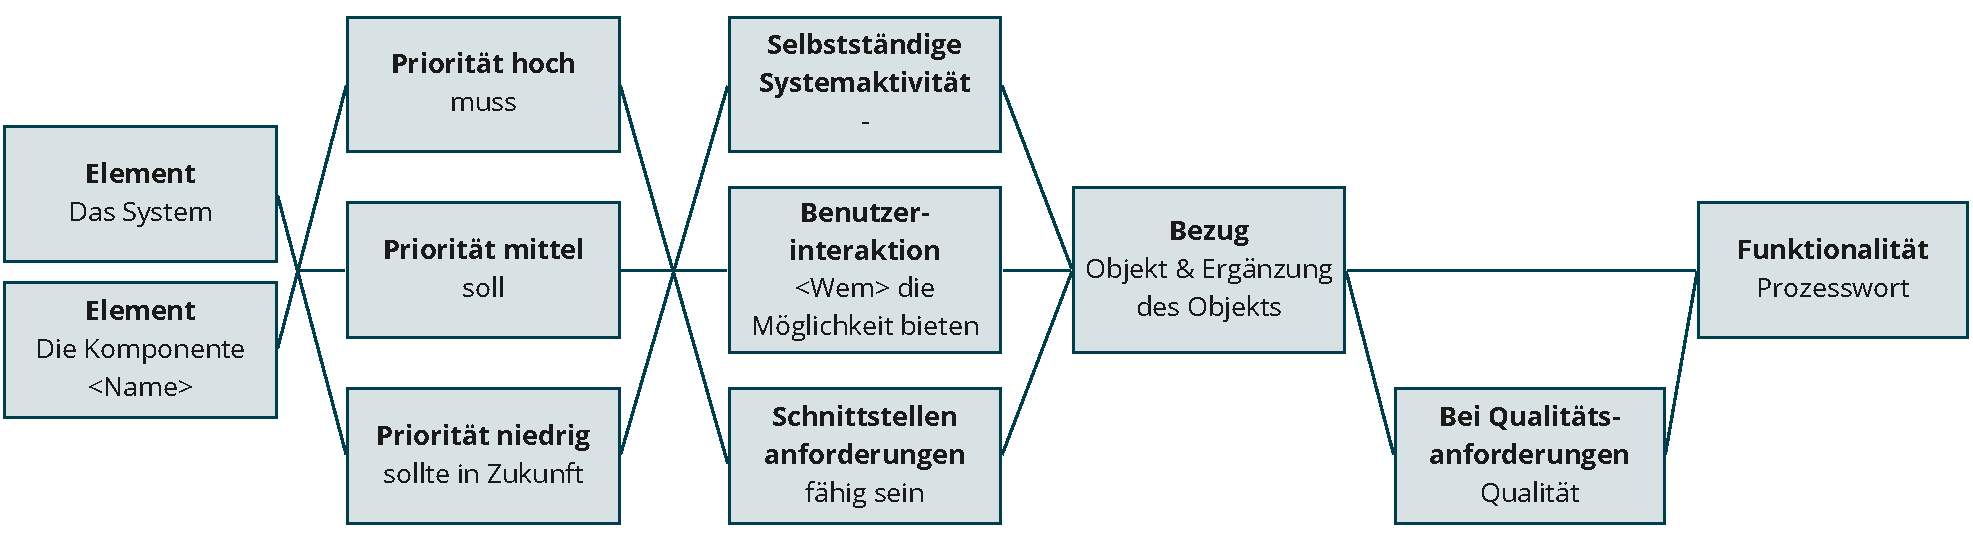
\includegraphics[scale=0.45]{Bilder/anforderungsschablone.pdf}
        \caption[Anforderungsschablone]{Anforderungsschablone \cite{Balzert2009}}
        \label{fig:schablone}
\end{figure}

\newpage
\setanf{F}
\begin{center}
        \renewcommand{\arraystretch}{1.5}
        \begin{longtable}{lp{0.85\textwidth}} \arrayrulecolor{maincolor}\hline
                \anfrow & Das System \textit{muss} Verleihenden und Ausleihenden die Möglichkeit
                bieten, alle Assets jederzeit mittels einer Übersicht einsehen zu können
                \textit{(Ag-Vt-1, \anfref{Z10})}.                                                  \\
                \anfrow & Das System \textit{muss} Verleihenden und Ausleihenden die Möglichkeit
                bieten, die Verfügbarkeit eines Assets einsehen zu können \textit{(Ag-Vt-2,
                \anfref{Z20})}.                                                                    \\
                \anfrow & Das System \textit{muss} Verleihenden und Ausleihenden die Möglichkeit
                bieten, nach Assets zu Filtern und zu Suchen.                                      \\
                \anfrow & Das System \textit{muss}  Verleihenden und Ausleihenden relevante
                Informationen zu den Assets anzeigen (Bild, Name, Beschreibung und Seriennummer)
                \textit{(Ag-Vt-4, Ag-Au-2, \anfref{Z20}, \anfref{Z40})}.
                \\
                \anfrow & Das System \textit{muss}  Ausleihenden relevante Informationen zu
                Ansprechpartner:innen anzeigen \textit{(Ag-Vt-4)}.
                \\
                \anfrow & Das System \textit{muss} Verleihenden und Ausleihenden die Möglichkeit
                bieten, Reservierungen von Assets vornehmen zu können \textit{(Ag-Vt-3)}.
                \\
                \anfrow & Das System \textit{muss} Verleihenden und Ausleihenden die Möglichkeit
                bieten, die verfügbaren Zeitslots der Assets einsehen zu können \textit{(Ag-Vt-2)}.
                \\
                \anfrow & Das System \textit{muss} Ausleihende daran erinnern, die ausgeliehenen
                Assets abzuholen, zurückzubringen oder zu verlängern sind \textit{(Ag-Au-1,
                Ag-Rg-1)}.                                                                         \\
                \anfrow & Das System \textit{soll} Verleihenden und Ausleihenden die Möglichkeit
                bieten, sich mit dem vorhanden IDM (LDAP) Account einzuloggen.
                \\
                \anfrow & Das System \textit{soll} Ausleihenden die Möglichkeit bieten, mittels
                einer Nutzen-Suche individuelle und personalisierte Asset-Vorschläge zu erhalten
                \textit{(Ag-Vt-3, Ag-Au-2)}.
                \\
                \anfrow & Das System \textit{soll} Verleihende automatisch kontaktieren, wenn ein
                Asset reserviert wurde (\textit{Ag-Vt-1}).
                \\
                \anfrow & Das System \textit{soll} Verleihende automatisch erinnern, wenn der
                Zugriff zu einem Asset benötigt wird (\textit{Ag-Au-1}).
                \\
                \anfrow & Das System \textit{soll} Verleihenden und Ausleihenden die Möglichkeit
                bieten, Mängel und Schäden am Asset zu Kennzeichen.
                \\
                \anfrow & Das System \textit{sollte in Zukunft} Verleihenden die Möglichkeit geben
                administrative Aufgaben zu erledigen und an Wartungen zu erinnern
                (\textit{Ag-Rg-2}).                                                                \\
                \anfrow & Das System \textit{sollte in Zukunft} Verleihenden und Ausleihenden die
                Möglichkeit bieten, Assets mithilfe eines QR-Scans in den Reservierung-Checkout zu
                packen.                                                                            \\
                \anfrow & Das System \textit{sollte in Zukunft} Verleihenden und Ausleihenden die
                Möglichkeit bieten, Kommentare und Erfahrungsberichte unter Assets zu schreiben.
                \\
                \anfrow & Das System \textit{sollte in Zukunft} Kommunikation mit Verleihenden
                ermöglichen, sodass keine extra Instanz benötigt wird.
                \\
                \arrayrulecolor{maincolor}\hline
        \end{longtable}
\end{center}

\vspace*{-1.5cm}
\subsection{Qualitätsanforderungen}
\label{section:qualität}
Im letzten Schritt werden die nicht-funktionalen Anforderungen festgelegt, welche die qualitativen
oder quantitativen Eigenschaften eines Systems darstellen \cite{Balzert2009}. Auch hier wird, falls
möglich, die Anforderungsschablone aus \ref{fig:schablone} verwendet.
\setanf{Q}
\begin{center}
        \renewcommand{\arraystretch}{1.5}
        \begin{longtable}{lp{0.85\textwidth}} \arrayrulecolor{maincolor}\hline
                \anfrow & Das System \textit{muss} den Grundsätzen der DIN EN ISO 9241-110:2019-09
                (Ergonomie der Mensch-System-Interaktion - Teil 110: Interaktionsprinzipien) folgen
                (\textit{DIN EN ISO 9241-110}, 2019).
                \\
                \anfrow & Das System \textit{muss} die definierten Nutzungsklassen aus
                \ref{section:benutzer} unterscheiden und die dazugehörigen Zugriffsrechte
                sicherstellen.                                                                       \\
                \anfrow & Das System \textit{muss} zuverlässig und ohne Störung im Dauerbetrieb
                laufen (\nameref{section:zeit}).                                                     \\
                \anfrow & Das System \textit{soll} modular strukturiert sein, damit Inhalte und
                Funktionalitäten effizient eingebunden werden können und das System einfach
                erweiterbar ist.                                                                     \\
                \anfrow & Das System \textit{soll} beim Zugriff über das Internet eine gesicherte
                Übertragung (bspw. \ac{HTTPS}) ermöglichen.
                \\
                \anfrow & Das System \textit{soll} alle Benutzerinteraktionen in unter fünf Sekunden
                ausführen.                                                                           \\
                \arrayrulecolor{maincolor}\hline
        \end{longtable}
\end{center}
